\documentclass[a4paper]{article}
\usepackage[ngerman]{babel}
\usepackage[T1]{fontenc}
\usepackage[utf8]{inputenc}
\usepackage{textcomp}
\usepackage{geometry}
\geometry{ left=2cm, right=2cm, top=2cm, bottom=4cm, bindingoffset=5mm}
\usepackage{graphicx}
\usepackage{xcolor}
\usepackage{hyperref}
\date{}
\author{}
\usepackage{fancyhdr}
\pagestyle{fancy}
\fancyhf{}
\fancyhead[R]{3141241 - Jamie Ullerich \\ xxxxxxx - Gerhard Breul \\ 2973140 - Felix Bühler}
\fancyhead[L]{Information Visualisation and Visual Analytics \\ WS 2019/20 }
\renewcommand{\headrulewidth}{0.5pt}

\title{Assignment 1}

\begin{document}
	\maketitle 
	\thispagestyle{fancy}
	
	\section*{Task 1 - Differences in visualization disciplines}
	
	Scientific visualisation focuses on 3D dimensional visualisations, like renderings of volumes, surface and isolines. 
	These should be realistic, since it is mostly used in medical applications, for biological or metrological reasons. 
	Additionally, there can be a time component and the layout is mostly given (or self explanatory).\\ \linebreak
	On the other hand, information visualisation focuses on abstract data, like networks, documents or statistics. 
	Since there is no natural analogy, the spatial layout must be chosen, in contrast to scientific applications. 
	Therefore the layout needs more explanation. 
	
	
	\section*{Task 2 - Historical Visualization}
	
	\begin{enumerate}
		\item[(a)] At the bottom of the graph, the temperature is shown. 
		Additionally, important geographical information, such as rivers or cities are displayed. The distance the army traveled is visible as well. 
		The third aspect is the size of the army, which is characterised by the thickness and numbers of the path. 
		The last  visualised aspect is the colour of the path, which is a brighter brown for the forward marching army and a darker brown for the returning soldiers. 
		\item[(b)] Yes, it is possible to automate this process. 
		Regarding the temperature, this can be visualised using temperature data available from weather stations.
		The landmarks are already available, as well, and the path can be constructed using the position of the army. 
		By using data about the size of the army, the thickness of the path can also be visualised. 
	\end{enumerate}
	
	\newpage
	\section*{Task 3 (Bonus Task) - Tag Cloud}
	\begin{figure}[!ht]
		\centering
		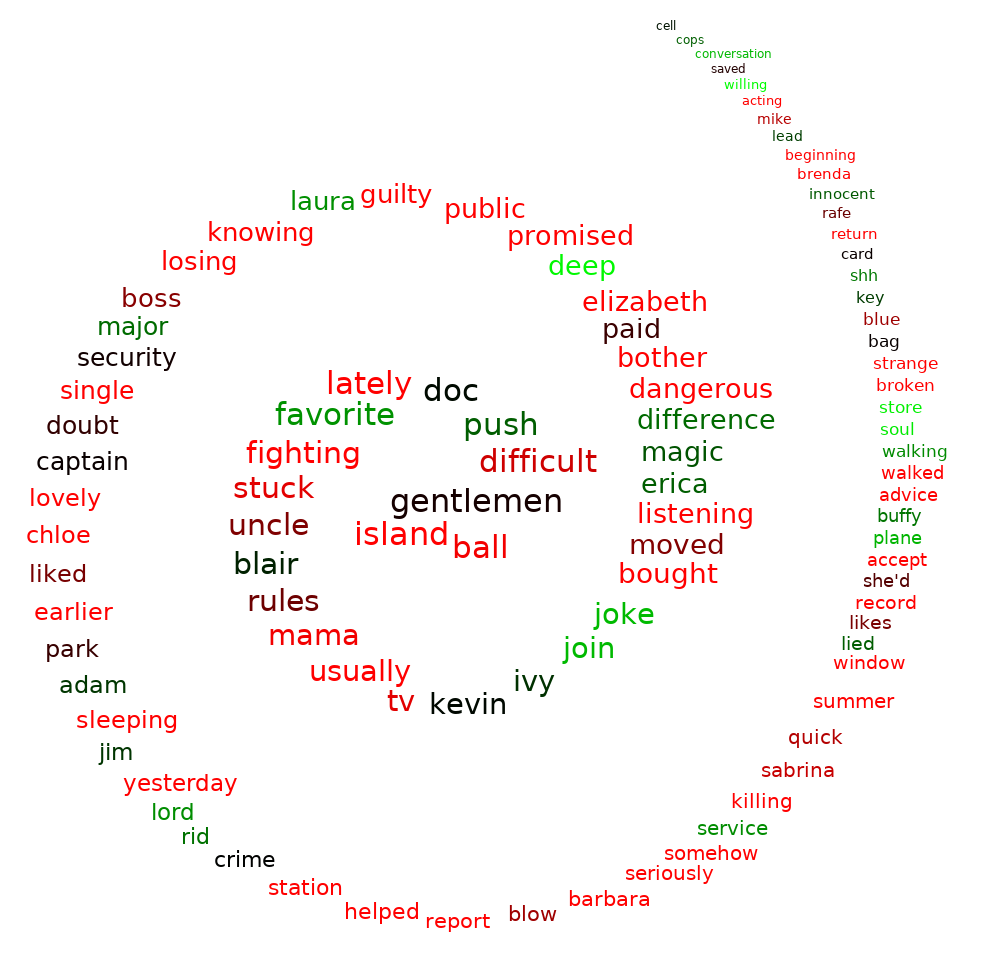
\includegraphics[width=0.7\linewidth]{1_3}
		\caption{result}
	\end{figure}
	
\end{document}
